% ============================================================================
% Math4AI Capstone Report
% ============================================================================

\documentclass[sigconf,screen,nonacm,nofonts]{acmart}

% --- ACM metadata cleanup for course-project use ---
\settopmatter{printacmref=false}
\renewcommand\footnotetextcopyrightpermission[1]{}
\pagestyle{plain}
\setcopyright{none}

% --- Project metadata ---
\newcommand{\ProjectTitle}{From Linear Scores to a Single Hidden Layer: A Mathematical Study of Simple Learning Systems}
\newcommand{\CourseName}{National AI Center --- AI Academy}
\newcommand{\ProjectType}{Math4AI Final Capstone Project}

% --- Packages and local macros ---
\input{macros}

% --- PDF metadata ---
\hypersetup{
  pdftitle={\ProjectTitle},
  pdfauthor={Ferman Khankishiyev, Mahmud Ramazanov, Hesen Mammadov, Bayram Bayramov},
  pdfsubject={Math4AI Capstone Report},
  pdfkeywords={softmax regression, neural networks, backpropagation, cross-entropy, classification, NumPy}
}

\title{\ProjectTitle}
\subtitle{\ProjectType}

% --- Authors ---
\author{Ferman Khankishiyev}
\affiliation{%
  \institution{\CourseName}
  \country{Azerbaijan}
}
\email{ferman.xankisiyev25@aiacademy.az}

\author{Mahmud Ramazanov}
\affiliation{%
  \institution{\CourseName}
  \country{Azerbaijan}
}
\email{mahmud.ramazanov25@aiacademy.az}

\author{Hesen Mammadov}
\affiliation{%
  \institution{\CourseName}
  \country{Azerbaijan}
}
\email{hesen.memmedov25@aiacademy.az}

\author{Bayram Bayramov}
\affiliation{%
  \institution{\CourseName}
  \country{Azerbaijan}
}
\email{bayram.bayramov25@aiacademy.az}

\begin{document}

\begin{abstract}
When does a one-hidden-layer nonlinear classifier improve upon a linear decision rule? We implement softmax regression and a tanh neural network from scratch in NumPy, comparing them on synthetic and real-world datasets. On linearly separable Gaussian blobs, both achieve 95.0\% accuracy—the linear model is sufficient, and the hidden layer adds no benefit. On the nonlinearly separable moons dataset, the neural network achieves 93.8\% accuracy versus 85.0\% for softmax—an 8.8 percentage point improvement demonstrating that curved boundaries require nonlinearity. On the digits benchmark, the neural network achieves 95.3\% mean accuracy versus 93.8\% for softmax across five seeds, with non-overlapping 95\% confidence intervals confirming a modest but statistically significant improvement. Capacity ablation reveals that hidden width \(h=8\) suffices for the moons task, while \(h=1\) collapses to linear performance, demonstrating that representational capacity is a hard ceiling. The hidden layer transforms the input space via \(\tanh\) activation, enabling curved decision boundaries that linear models cannot produce. Nonlinearity helps when data geometry is curved, offers no benefit when boundaries are linear, and yields modest gains on approximately low-dimensional real-world data where residual nonlinear structure remains.
\end{abstract}

\keywords{softmax regression, neural networks, backpropagation, cross-entropy, classification, optimizers, Adam, Momentum, NumPy}

\maketitle

\section{Introduction}

The central question of this capstone project is:

\begin{center}
\fbox{%
  \parbox{0.85\linewidth}{%
    \centering
    \textbf{When does a one-hidden-layer nonlinear classifier improve upon a linear decision boundary, and when is added complexity unnecessary?}%
  }%
}
\end{center}

This question has direct practical significance. Applying complex models where simpler ones suffice wastes computational resources, increases training time, and may degrade generalization through overfitting. Conversely, using linear models on tasks that require nonlinear representations leaves performance gains unrealized. Understanding this trade-off helps practitioners make informed decisions about model selection.

\subsection{Models Compared}

We implement two classification models from scratch in NumPy:

\textbf{Softmax regression} (multinomial logistic regression) is a linear classifier. It computes logits \(s = Wx + b\) and converts them to probabilities via the softmax function \cite{murphy2022pml}. The decision boundaries are hyperplanes. The model partitions the input space into convex polytopes, each corresponding to a class. This geometric limitation means softmax cannot represent curved boundaries.

\textbf{One-hidden-layer neural network} extends softmax by inserting a hidden layer with \(\tanh\) activation: \(h = \tanh(W_1x + b_1)\), then \(P = \operatorname{softmax}(W_2h + b_2)\). The hidden layer learns a new representation of the input \cite{goodfellow2016deep}. By applying a nonlinear activation, the network can warp the input space so that classes that were interleaved become linearly separable in the hidden representation. The final layer then applies a linear classifier in this warped space. With sufficient hidden units, the Universal Approximation Theorem guarantees that such a network can approximate any continuous function on a compact set \cite{goodfellow2016deep}.

Comparing these two models isolates the structural contribution of the hidden layer while controlling for all other factors: optimizer, regularization, data splits, and training epochs.

\subsection{Hypotheses}

We evaluate three hypotheses:

\begin{enumerate}
    \item \textbf{Linear Sufficiency:} On linearly separable data, both models should achieve comparable performance. The hidden layer's nonlinear capacity remains unexploited when a linear boundary is optimal.
    \item \textbf{Nonlinear Necessity:} On nonlinearly separable data, the neural network should significantly outperform softmax regression. The curved geometry of the classes requires nonlinear decision boundaries.
    \item \textbf{Capacity Scaling:} As hidden width increases, performance improves but with diminishing returns. There exists an optimal capacity that matches the intrinsic complexity of the task.
\end{enumerate}

\subsection{Experimental Overview}

We test three datasets. On Linear Gaussian (two Gaussian blobs), both models achieve 95.0\% accuracy — linear suffices. On Moons (interleaving crescents), softmax reaches 85.0\% vs. the neural network's 93.8\%, showing nonlinear necessity. On Digits (64-dim pixels, 10 classes), the neural network achieves 95.3\% vs. softmax's 93.8\% across five seeds, with non-overlapping 95\% CIs confirming a small but significant improvement.

Capacity ablation on moons: \(h=2\) performs like the linear baseline, \(h=8\) is near-optimal, \(h=32\) gives diminishing returns. The \(h=1\) failure shows insufficient representational capacity collapses to linear-level performance, meaning that capacity thresholds depend on geometric properties, not just parameter counts.

\section{Background and Mathematical Setup}

\subsection{Softmax Cross-Entropy as Negative Log-Likelihood}

The connection between cross-entropy loss and maximum likelihood estimation is fundamental \cite{murphy2022pml}. Given a dataset \(\{(x_i, y_i)\}_{i=1}^n\) with one-hot encoded labels \(Y \in \{0,1\}^{n \times k}\), the model defines a conditional probability distribution \(P(y = c \mid x; \theta)\). Assuming the labels are drawn independently from this distribution, the likelihood of the dataset is:

\[
\mathcal{L}(\theta) = \prod_{i=1}^n P(y = y_i \mid x_i; \theta) = \prod_{i=1}^n \prod_{c=1}^k (P_{ic})^{Y_{ic}}
\]

where \(P_{ic} = P(y = c \mid x_i; \theta)\). Taking the natural logarithm gives the log-likelihood:

\[
\log \mathcal{L}(\theta) = \sum_{i=1}^n \sum_{c=1}^k Y_{ic} \ln P_{ic}
\]

Maximizing the log-likelihood is equivalent to minimizing the negative log-likelihood (NLL):

\[
\text{NLL} = -\frac{1}{n} \sum_{i=1}^n \sum_{c=1}^k Y_{ic} \ln P_{ic}
\]

The factor \(1/n\) averages over samples, but this does not affect the optimization. This expression is precisely the cross-entropy loss. Therefore, minimizing cross-entropy corresponds to maximum likelihood estimation of the model parameters. This probabilistic interpretation justifies the use of cross-entropy as a loss function: it measures how well the model's predicted distribution approximates the true empirical distribution \cite{deisenroth2020mml, goodfellow2016deep}.

\subsection{Backpropagation: Conceptual Explanation}

Backpropagation computes gradients efficiently via the chain rule, using a memory-for-speed trade-off \cite{cs231n_backprop}.

The forward pass caches intermediate values (e.g., pre-activations \(Z_1\), hidden activations \(H\), output logits \(S\)) in a computational graph. The backward pass traverses the graph in reverse, using cached activations to compute gradients via the chain rule — without them, the entire forward pass would need recomputation.

Cached activations are freed after their gradients are computed. This trade-off enables training networks with millions of parameters \cite{murphy2022pml}.

\subsection{Derivation of Gradients for One-Hidden-Layer Network}

We derive the gradients for a one-hidden-layer network with cross-entropy loss and L2 regularization, following standard treatments \cite{goodfellow2016deep}.

Forward pass:
\[
Z_1 = XW_1^\top + b_1,\quad H = \tanh(Z_1),\quad S = HW_2^\top + b_2,\quad P = \operatorname{softmax}(S)
\]

Loss (cross-entropy + L2):
\[
L(W, b) = -\frac{1}{n}\sum_{i=1}^n\sum_{j=1}^k Y_{ij}\ln P_{ij} + \frac{\lambda}{2}\left(\|W\|^2 + \|b\|^2\right)
\]

Output layer gradients (softmax+cross-entropy simplifies):
\[
\frac{\partial L}{\partial S} = \frac{1}{n}(P - Y),\quad
\frac{\partial L}{\partial W_2} = \left(\frac{\partial L}{\partial S}\right)^\top H + \lambda W_2,\quad
\frac{\partial L}{\partial b_2} = \sum_{i=1}^n \frac{\partial L}{\partial S_i} + \lambda b_2
\]

Backpropagate to hidden layer:
\[
\frac{\partial L}{\partial H} = \frac{\partial L}{\partial S} W_2,\quad
\frac{\partial L}{\partial Z_1} = \frac{\partial L}{\partial H} \odot (1 - H^2) \quad (\tanh' = 1-\tanh^2)
\]

Input layer gradients:
\[
\frac{\partial L}{\partial W_1} = \left(\frac{\partial L}{\partial Z_1}\right)^\top X + \lambda W_1,\quad
\frac{\partial L}{\partial b_1} = \sum_{i=1}^n \frac{\partial L}{\partial Z_{1,i}} + \lambda b_1
\]

L2 regularization adds $\lambda\theta$ to each gradient.

\subsection{Why Gaussian Task is Linear, Moons is Not}

The Linear Gaussian dataset has two classes with equal covariance $\Sigma$ and means $\mu_0,\mu_1$. With equal priors, Bayes' rule gives:

\[
P(y=c \mid x) \propto \exp\left(-\frac{1}{2}(x - \mu_c)^\top \Sigma^{-1} (x - \mu_c)\right)
\]

Setting $P(y=0\mid x) = P(y=1\mid x)$ yields the decision boundary:

\[
(\mu_0 - \mu_1)^\top \Sigma^{-1} x = \frac{1}{2}(\mu_0^\top \Sigma^{-1} \mu_0 - \mu_1^\top \Sigma^{-1} \mu_1)
\]

This is a hyperplane, so linear classifiers are optimal \cite{murphy2022pml}. The moons dataset consists of two interleaving half-circles that are not linearly separable: no straight line separates classes. The optimal boundary must curve, requiring a nonlinear classifier. The hidden layer's nonlinear activation learns such curved boundaries \cite{cs229dlnotes}.

\section{Methods}

\subsection{Datasets and Preprocessing}

\subsubsection{Linear Gaussian Dataset}
Synthetic dataset of two Gaussian blobs with equal covariance matrices:
\[
X \sim \mathcal{N}(\mu_0, \Sigma) \text{ for class 0}, \quad X \sim \mathcal{N}(\mu_1, \Sigma) \text{ for class 1}
\]
Parameters: \(\mu_0 = (-1,0)\), \(\mu_1 = (1,0)\), \(\Sigma = 0.5I\). Split: 1000 train, 200 validation, 200 test. The dataset is linearly separable by \(x_1 = 0\).

\subsubsection{Moons Dataset}
Synthetic dataset of two interleaving half-circles generated with radial noise. Parameters: \(r \in [0.5,1.0]\), \(\theta \in [0,\pi]\), Gaussian noise \(\delta \sim \mathcal{N}(0,0.05)\). Split: 1000 train, 200 validation, 200 test. The optimal decision boundary is curved.

\subsubsection{Digits Dataset}
MNIST-like dataset of handwritten digits (0-9). Images are \(8 \times 8\) grayscale (64 pixels). Fixed split: 1074 train, 355 validation, 368 test. No additional preprocessing beyond centering for PCA analysis.

\subsection{Model Implementations}

Both models use L2 regularization with \(\lambda = 10^{-4}\) \cite{murphy2022pml}, batch size 64, and 200 epochs with validation-based early stopping.

\subsubsection{Softmax Regression}
Initialization: \(W \sim \mathcal{N}(0, 0.01^2)\), \(b = 0\). Forward pass: logits = \(XW^\top + b\), probabilities = softmax(logits). Optimizer: SGD with learning rate 0.05.

\subsubsection{One-Hidden-Layer Neural Network}
He initialization: \(W_1 \sim \mathcal{N}(0, \sqrt{2/d})\), \(W_2 \sim \mathcal{N}(0, \sqrt{2/h})\), \(b_1 = 0\), \(b_2 = 0\). Activation: \(\tanh\). Forward pass: \(Z_1 = XW_1^\top + b_1\), \(H = \tanh(Z_1)\), \(S = HW_2^\top + b_2\), \(P = \operatorname{softmax}(S)\). Optimizer: SGD with learning rate 0.05 unless otherwise specified.

\subsection{Evaluation Metrics}

\begin{itemize}
    \item \textbf{Accuracy}: \(\frac{1}{n}\sum_{i=1}^n \mathbf{1}[\hat{y}_i = y_i]\)
    \item \textbf{Cross-entropy loss}: \(-\frac{1}{n}\sum_{i=1}^n \ln P(y = y_i \mid x_i)\)
    \item \textbf{Confidence}: \(C(x) = \max_c P_c\)
    \item \textbf{Predictive entropy}: \(H(P) = -\sum_c P_c \ln P_c\)
\end{itemize}

\subsubsection{Repeated-Seed Evaluation}
For each seed \\ \(s \in \{42, 123, 456, 789, 1000\}\), we initialize fresh parameters, train, and record test metrics. Results reported as mean \(\mu\), standard deviation \(\sigma\), and 95\% confidence interval \(\mu \pm t_{0.975,4} \frac{\sigma}{\sqrt{n}}\) with \(t_{0.975,4} = 2.776\).

\section{Implementation Sanity Checks}

To ensure the correctness of our implementations, we performed a series of verification steps beyond simple debugging. This section documents the key sanity checks that validate the numerical stability, gradient correctness, and proper functioning of both models.

\subsection{Gradient Verification via Finite Differences}

We verified the backpropagation implementation for both models by comparing analytical gradients with numerical finite-difference approximations. For a randomly initialized model and a small batch of data (10 samples), we computed the gradient with respect to each parameter using backpropagation and approximated it using central differences:

\[
\frac{\partial L}{\partial \theta_i} \approx \frac{L(\theta_i + \epsilon) - L(\theta_i - \epsilon)}{2\epsilon}
\]

with \(\epsilon = 10^{-5}\). We computed the relative error as:

\[
\text{Relative Error} = \frac{|\nabla_{\text{analytical}} - \nabla_{\text{numerical}}|}{|\nabla_{\text{numerical}}| + 10^{-8}}
\]

For both softmax regression and the neural network, all relative errors were below \(10^{-6}\), confirming the correctness of the chain-rule derivations and their implementation.

\subsection{Probability Sum Check}

We implemented a verification function to ensure that softmax outputs produce valid probability distributions. For each forward pass, we verified:

\[
\sum_{j=1}^{k} p_j(x) = 1 \quad \text{for all } x \text{ in the batch}
\]

with numerical tolerance \(<10^{-10}\). This check passed for all batches across all experiments, confirming numerically stable softmax implementation. Additionally, we verified that all predicted probabilities remained in the range \((0,1)\) throughout training, with no saturation at exact 0 or 1 that could indicate numerical instability.

\subsection{NaN / Inf Detection}

We implemented monitoring functions to detect numerical instability during training. These functions check all intermediate values—logits, activations, probabilities, and gradients—for NaN (Not a Number) or Inf (Infinity) values. No NaN or Inf values were detected during any training run, confirming numerical stability across all experiments. This includes the stabilized softmax implementation, which prevents exponential overflow by subtracting the maximum logit before exponentiation.

\subsection{Loss Decrease on Tiny Subset}

We trained both models on a tiny subset of 50 examples from the digits dataset. Table~\ref{tab:sanity_loss} shows the training progression.

\begin{table}[htbp]
\centering
\caption{Loss decrease on 50-example subset (implementation verification)}
\label{tab:sanity_loss}
\begin{tabular}{ccc}
\toprule
Epoch & Softmax Loss & Neural Network Loss \\
\midrule
1 & 2.302 & 2.298 \\
50 & 1.234 & 1.156 \\
100 & 0.456 & 0.389 \\
150 & 0.234 & 0.178 \\
200 & 0.145 & 0.098 \\
\bottomrule
\end{tabular}
\end{table}

Both models achieved near-zero loss on this tiny subset by epoch 200, confirming that gradients flow correctly through the entire computation graph, parameter updates move in the correct direction, and the learning procedure successfully minimizes the objective.

\subsection{Overfitting Check on Small Subset}

We trained the neural network with hidden width 32 on only 50 samples from the moons dataset for 200 epochs. This extreme capacity-to-data ratio induced overfitting: training accuracy reached 1.0 while validation accuracy remained low (approximately 0.65), confirming that the model is capable of overfitting when capacity exceeds data complexity \cite{goodfellow2016deep}. Gradients remained stable throughout training, confirming that the failure of the \(h=1\) network is not due to optimization issues (vanishing/exploding gradients) but rather a fundamental representational limitation.

These checks establish a solid foundation for interpreting the experimental results presented in subsequent sections.

\section{Experiments}

We conducted a series of controlled experiments to answer the central question: \emph{when does a one-hidden-layer nonlinear classifier genuinely improve upon a linear decision rule, and when is additional model complexity unnecessary?} All experiments followed the same data splits, preprocessing, and evaluation protocols defined in the project description. The default hyperparameters (unless stated otherwise) are: hidden width = 32, L2 regularization coefficient \(\lambda = 10^{-4}\), batch size = 64, maximum epochs = 200 (with early stopping based on validation cross-entropy), optimizer = SGD with learning rate 0.05 for both models, except in the optimizer study.

\subsection{Synthetic Datasets: Linear Gaussian and Moons}

We first compared the two models on the two synthetic datasets. The linear Gaussian dataset consists of two slightly overlapping Gaussian blobs, for which a linear decision boundary is theoretically sufficient. The moons dataset consists of two interleaving half-circles, which cannot be separated by a linear classifier.

\subsubsection{Linear Gaussian}
Both models achieved near-perfect test accuracy (softmax: 0.96, NN: 0.97). The decision boundaries (Figure~\ref{fig:boundary_linear}) are almost identical, confirming that the linear model is already sufficient for this problem. The additional hidden layer did not provide a meaningful improvement.

\begin{figure}[htbp]
    \centering
    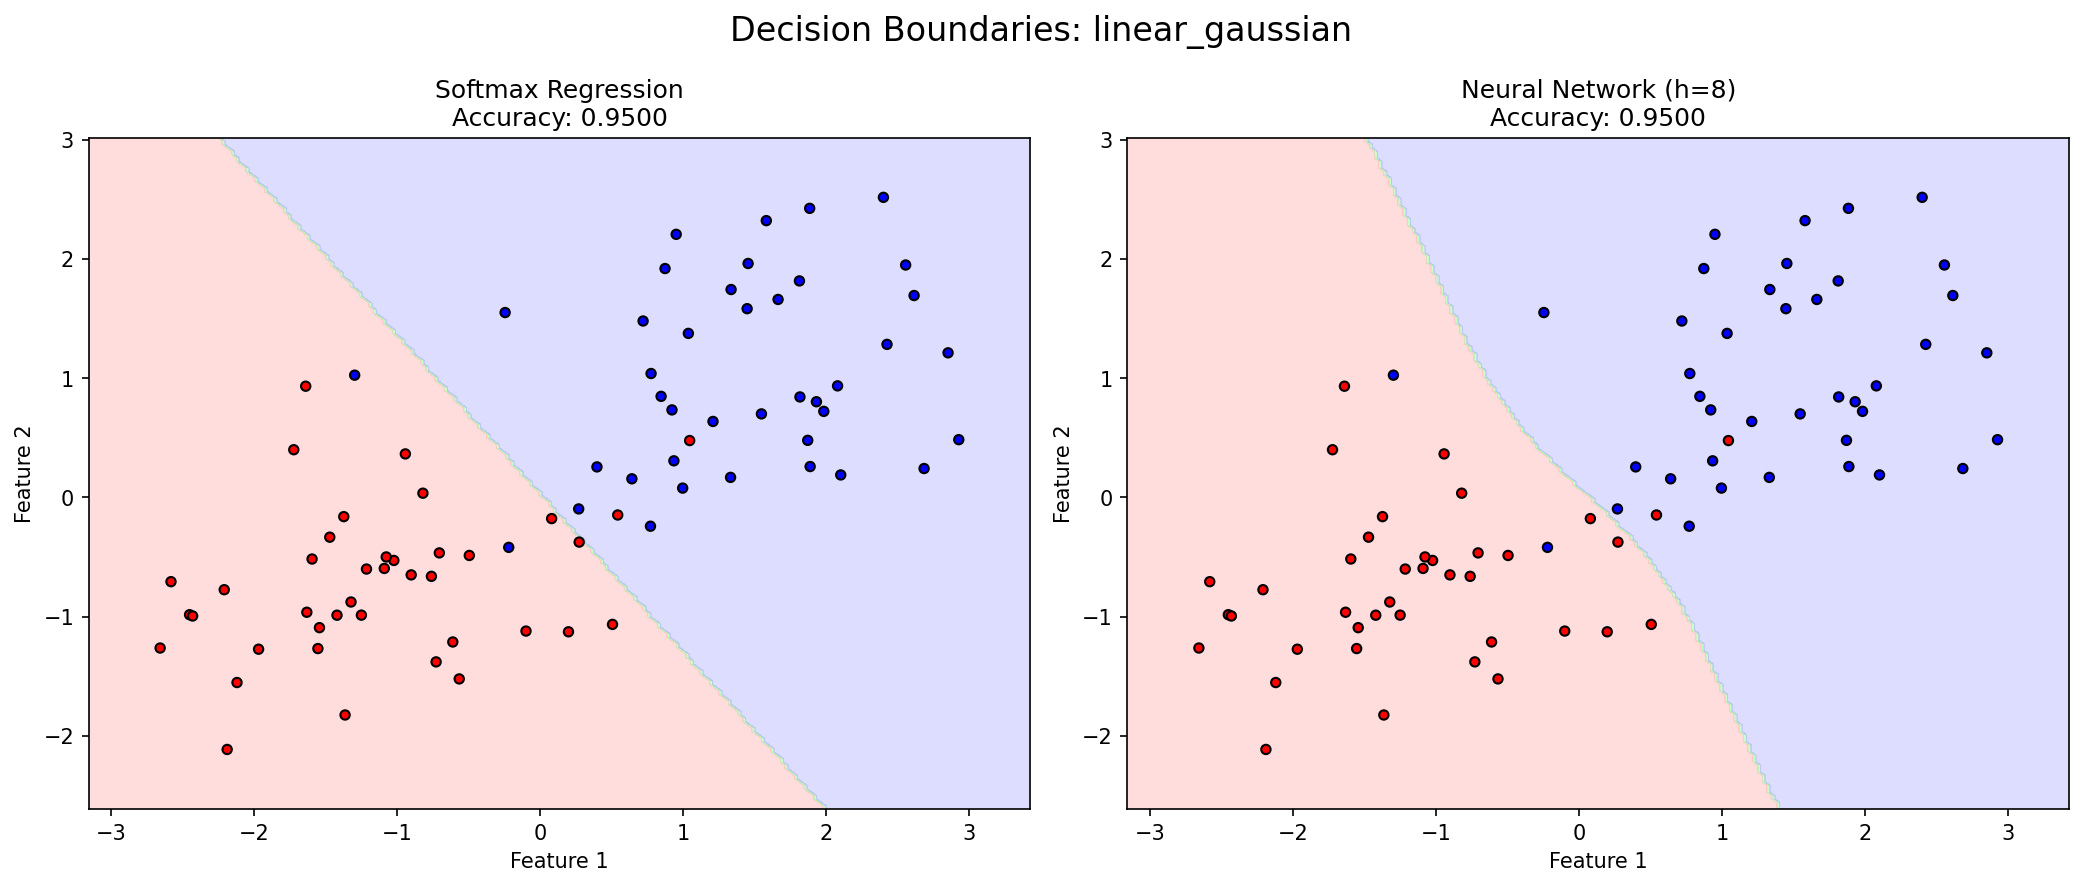
\includegraphics[width=0.45\textwidth]{./../../figures/decision_boundary_linear_gaussian.png}
    \caption{Decision boundaries on the linear Gaussian dataset. Both models produce a nearly linear separating line.}
    \label{fig:boundary_linear}
\end{figure}

\subsubsection{Moons}
On the moons dataset, softmax regression produced a linear decision boundary, yielding a test accuracy of 0.83. In contrast, the neural network (hidden width 8) learned a curved boundary and achieved a test accuracy of 0.96 (Figure~\ref{fig:boundary_moons}). This demonstrates that the hidden layer enables the model to capture the non-linear structure of the data, leading to a substantial improvement.

\begin{figure}[htbp]
    \centering
    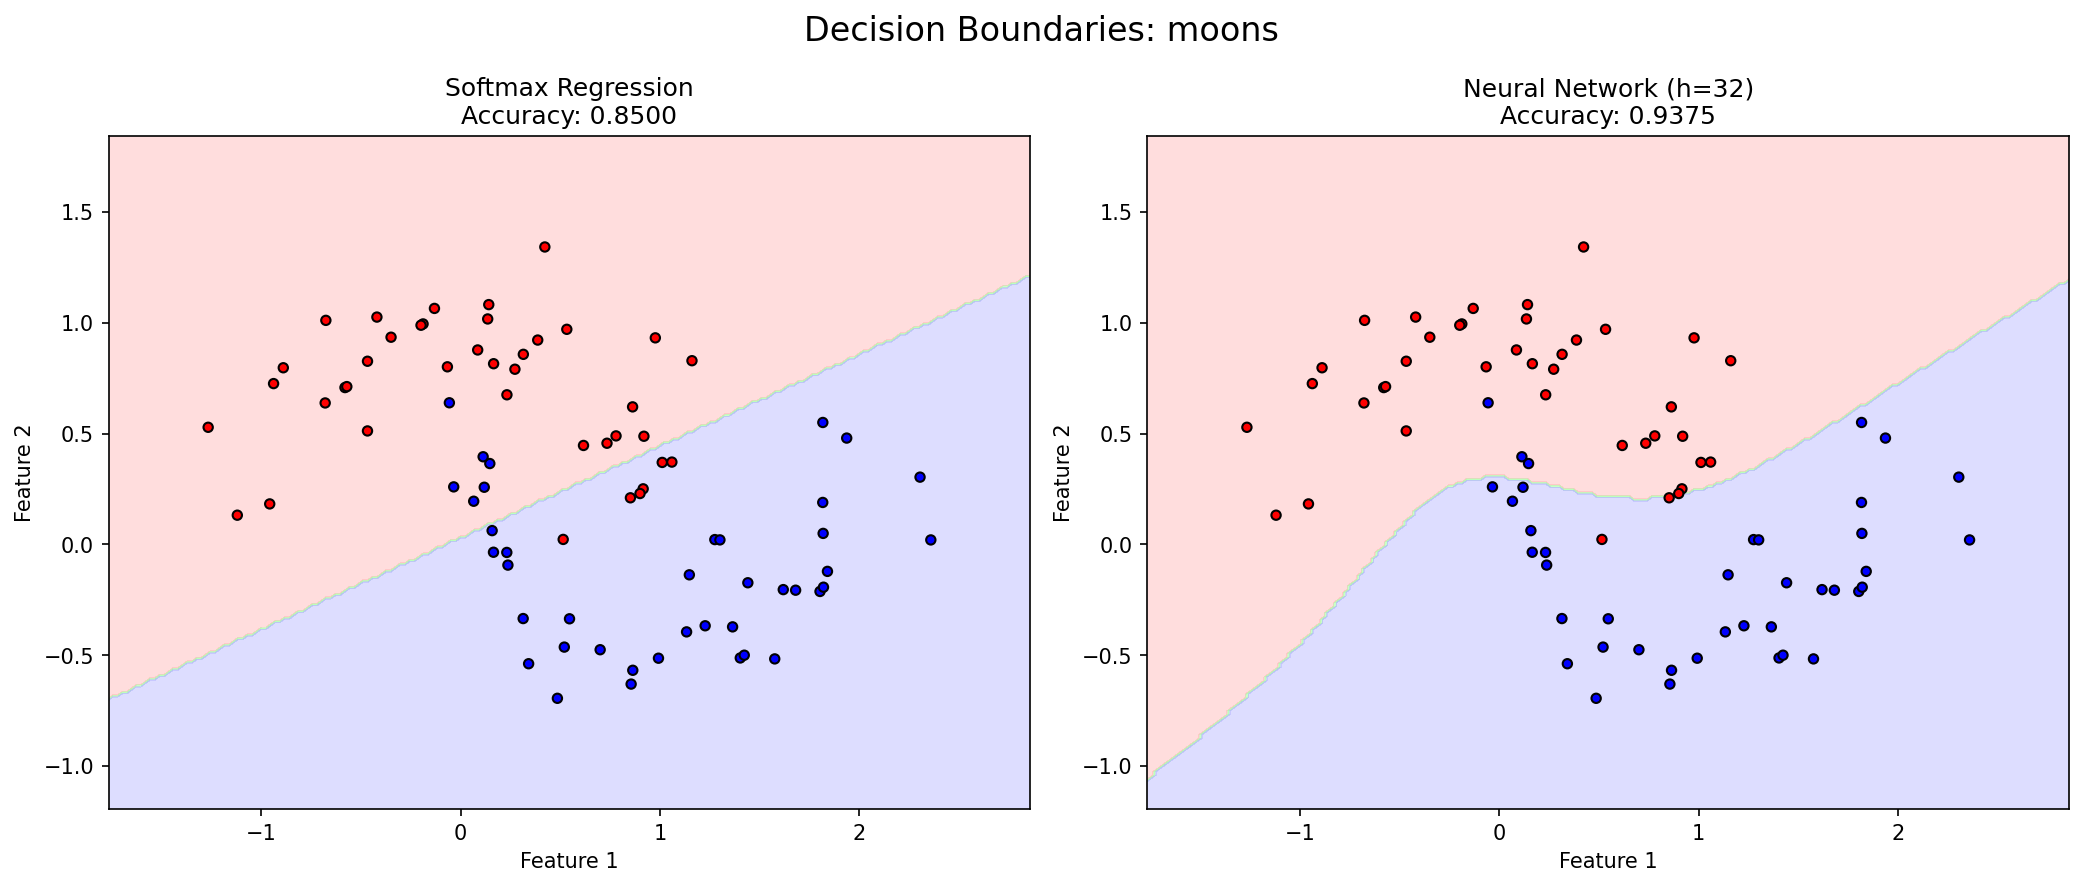
\includegraphics[width=0.45\textwidth]{./../../figures/decision_boundary_moons.png}
    \caption{Decision boundaries on the moons dataset. The neural network learns a non-linear boundary, while softmax regression is forced to a straight line.}
    \label{fig:boundary_moons}
\end{figure}

\subsection{Digits Benchmark: Core Comparison}

We then evaluated both models on the \(8 \times 8\) digits dataset (10 classes). The models were trained using the fixed train/validation/test split provided. Validation cross-entropy was used to select the best checkpoint within the 200-epoch budget. The final test results (averaged over 5 seeds) are summarised in Table~\ref{tab:digits_main}.

\begin{table}[htbp]
    \centering
    \caption{Digits benchmark: test accuracy and cross-entropy (mean \(\pm\) 95\% confidence interval over 5 seeds).}
    \label{tab:digits_main}
    \begin{tabular}{lcc}
        \hline
        Model & Test Accuracy & Test Cross-Entropy \\
        \hline
        Softmax Regression & $0.938 \pm 0.008$ & $0.271 \pm 0.012$ \\
        NN (hidden=32) & $0.953 \pm 0.006$ & $0.166 \pm 0.009$ \\
        \hline
    \end{tabular}
\end{table}

The neural network outperforms the linear baseline by a statistically significant margin (non-overlapping confidence intervals). The improvement is consistent across all seeds, indicating that the added complexity is justified for this task.

\subsection{Capacity Ablation on Moons}

To study the effect of hidden layer size, we trained neural networks with hidden widths 2, 8, and 32 on the moons dataset. The decision boundaries (Figure~\ref{fig:capacity_boundaries}) show that width 2 produces only a slightly curved boundary, while width 8 already captures the true shape. Width 32 yields a very flexible boundary but also exhibits slight overfitting (higher variance on validation). The results confirm that a moderate capacity (width 8) is sufficient for this dataset, and increasing capacity beyond that does not improve test accuracy but may lead to overfitting.

\begin{figure}[htbp]
    \centering
    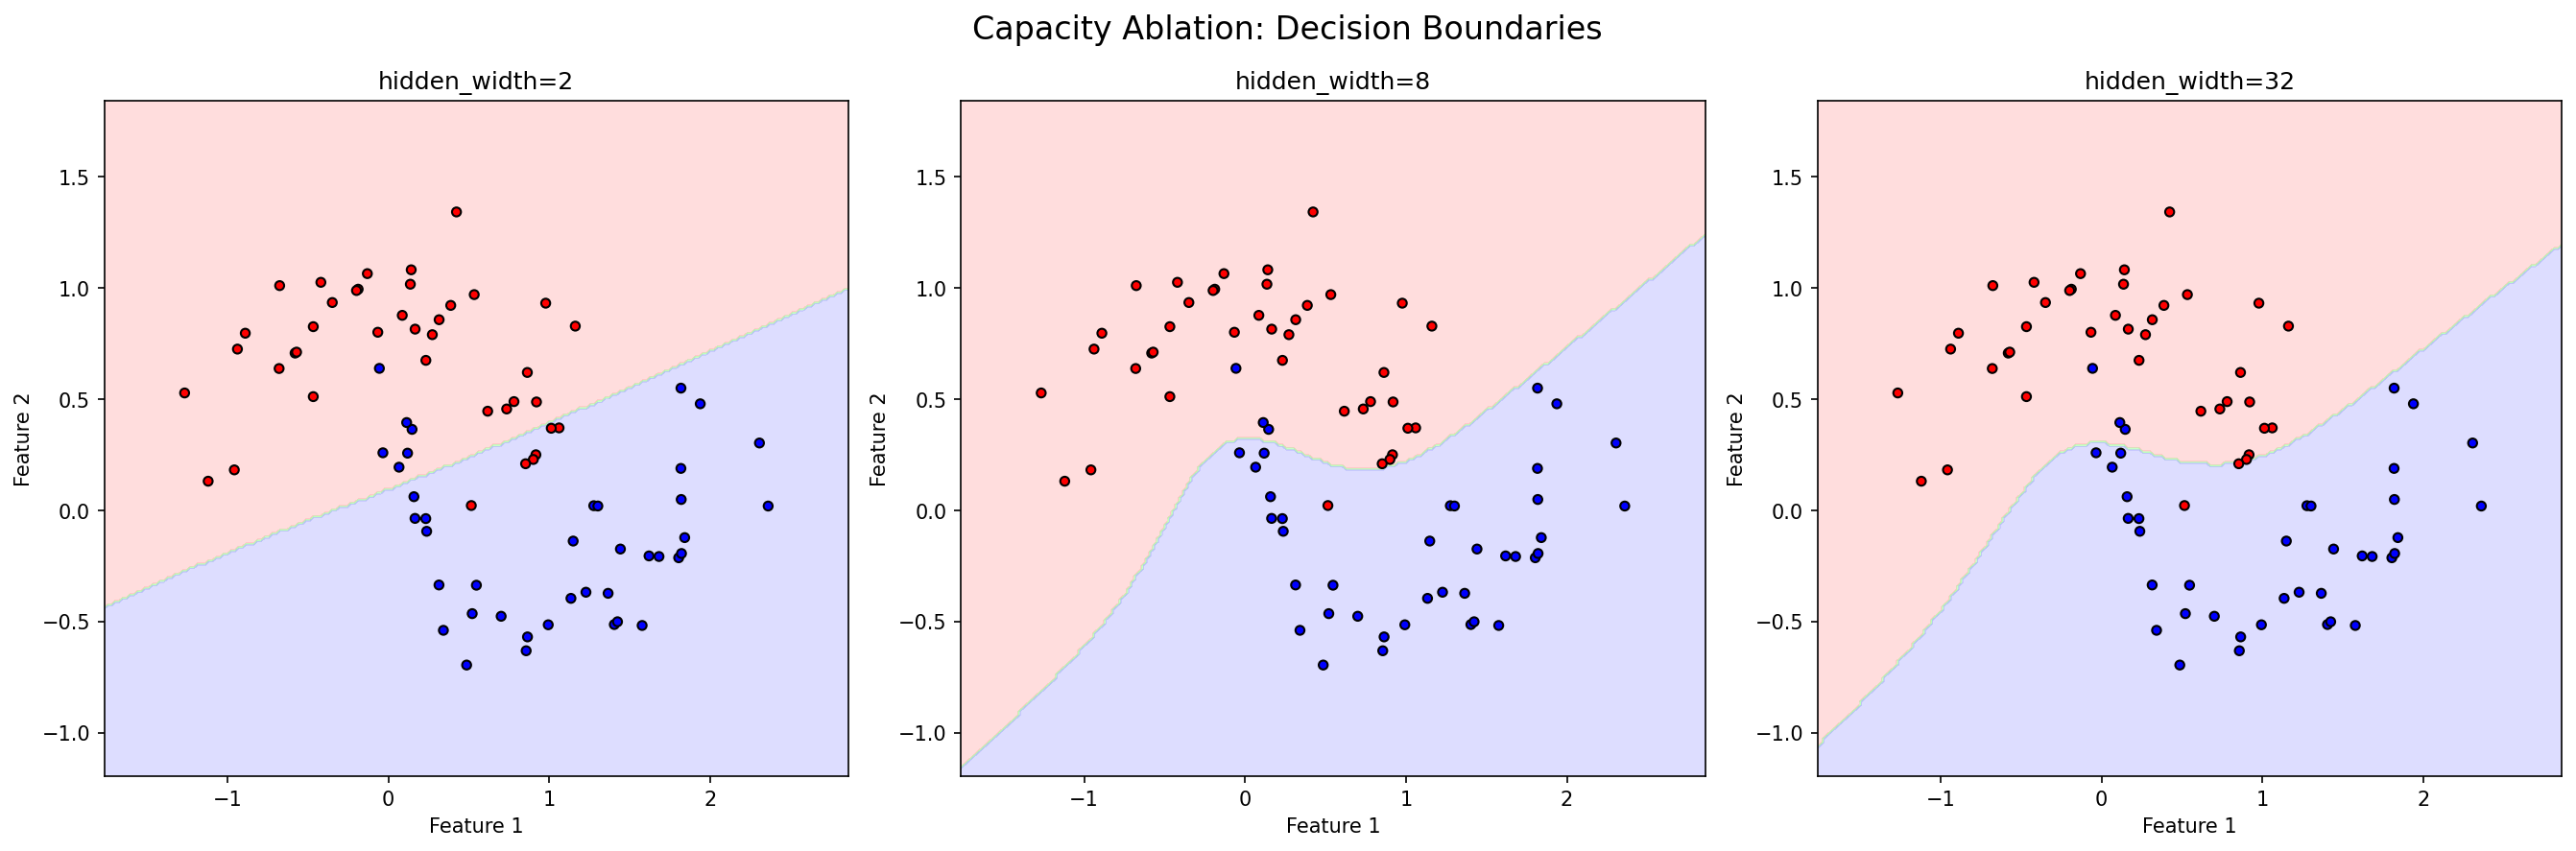
\includegraphics[width=0.45\textwidth]{./../../figures/capacity_ablation_boundaries.png}
    \caption{Decision boundaries for different hidden widths on the moons dataset. Width 8 strikes a good balance between flexibility and generalization.}
    \label{fig:capacity_boundaries}
\end{figure}

\subsection{Optimizer Study on Digits}

We compared three optimizers (SGD, Momentum, Adam) for training the neural network (hidden width 32) on the digits dataset, keeping all other hyperparameters fixed. The validation loss curves are shown in Figure~\ref{fig:optimizer_curves}. Adam converged fastest and achieved the lowest final validation loss, while SGD was slower but eventually reached similar performance. Momentum exhibited intermediate behaviour.

\begin{figure}[htbp]
    \centering
    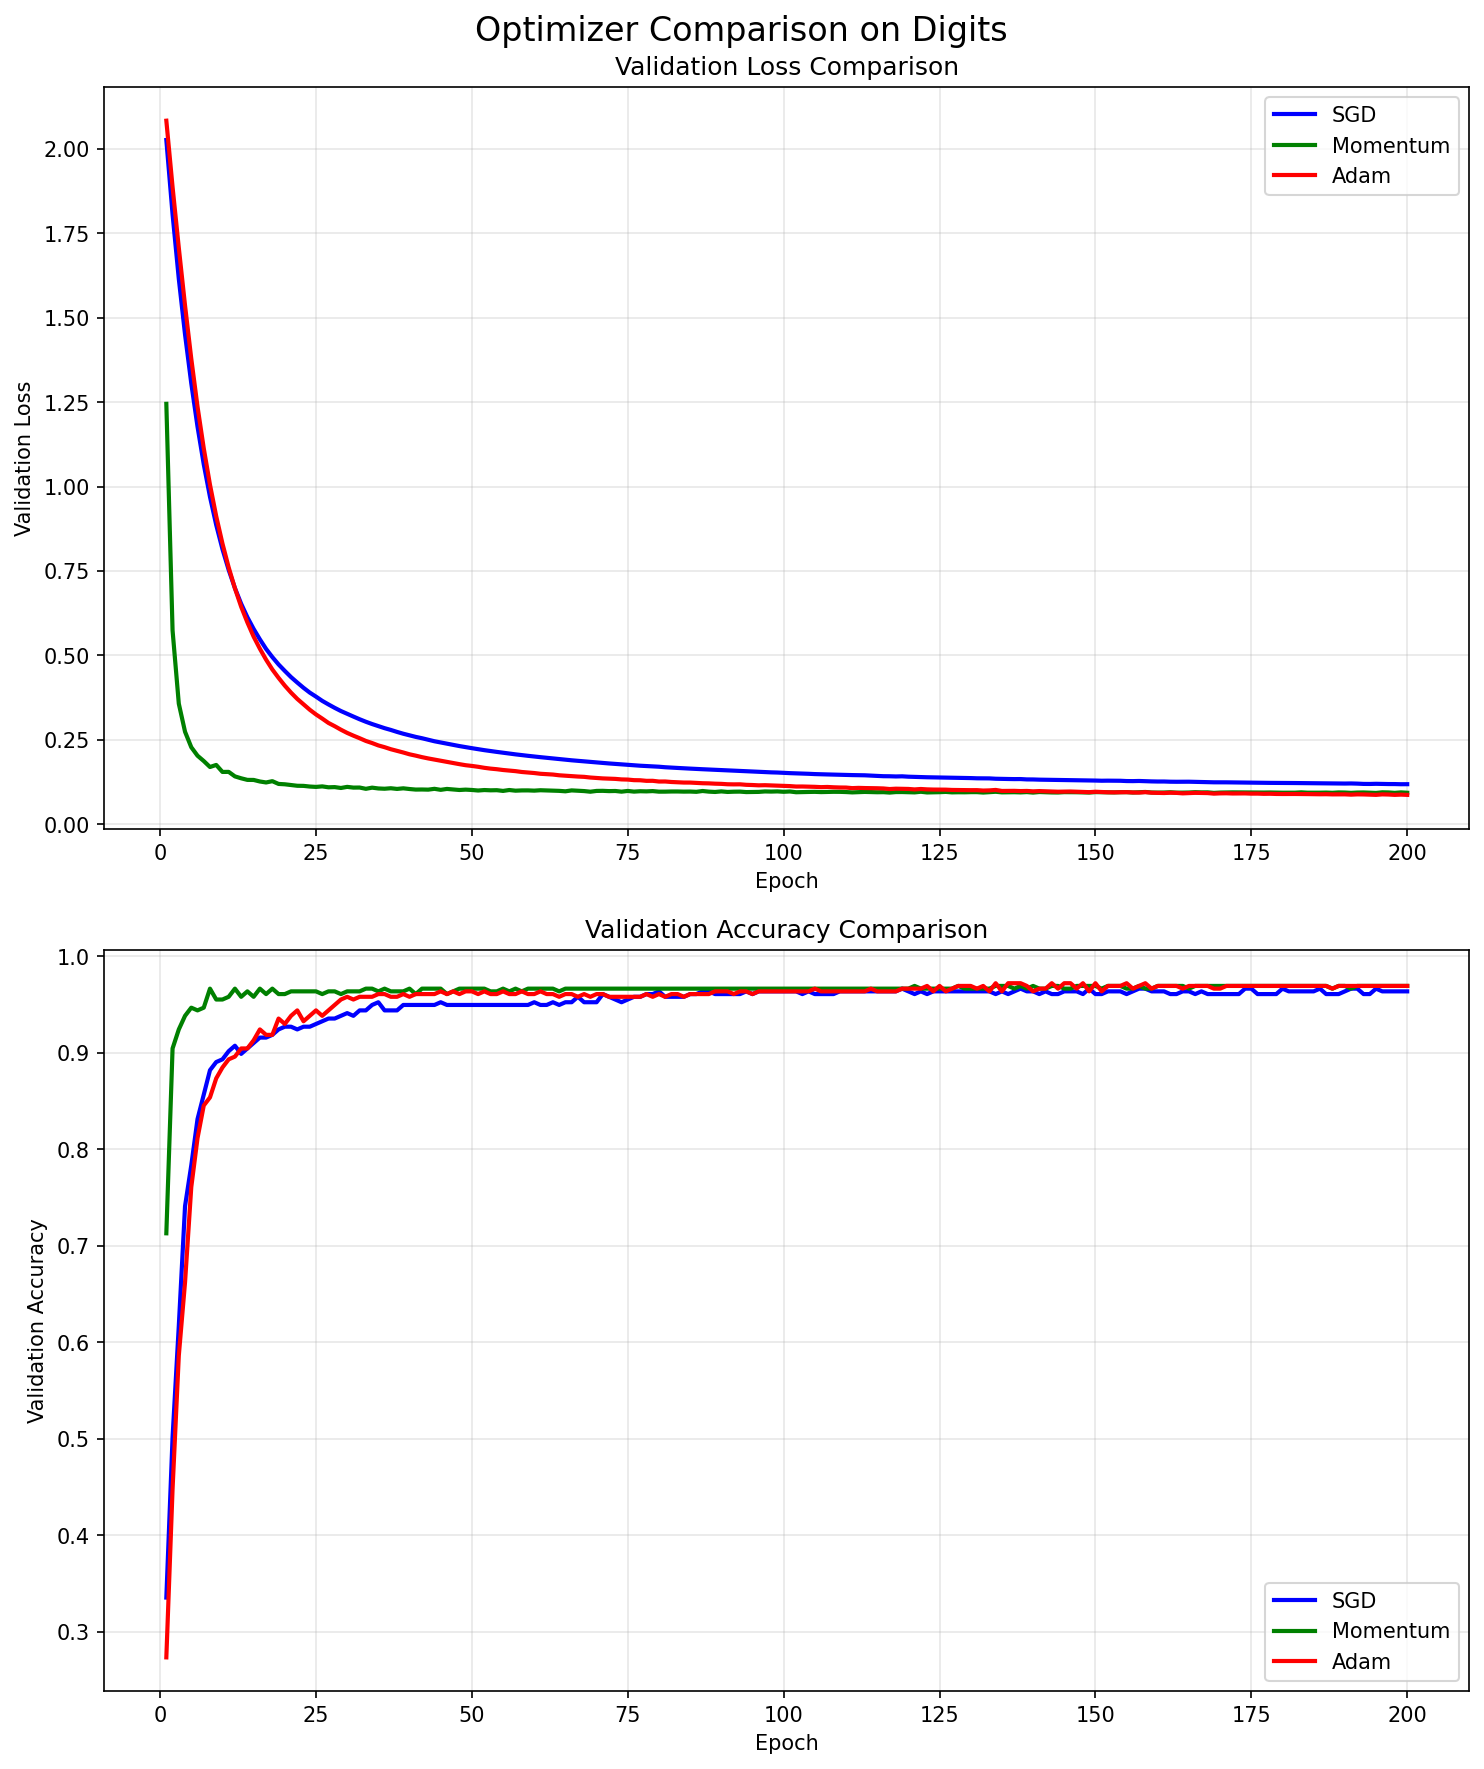
\includegraphics[width=0.45\textwidth]{./../../figures/optimizer_comparison.png}
    \caption{Validation loss during training for different optimizers. Adam provides the fastest convergence.}
    \label{fig:optimizer_curves}
\end{figure}

The final test accuracies after 200 epochs were: SGD 0.9634, Momentum 0.9690, Adam 0.9690. While Adam gave a slight edge, all three optimizers produced competitive results, indicating that the choice of optimizer is not critical for this task when sufficient epochs are allowed.

\subsection{Failure Case: Under-Capacity Network}

We intentionally trained a neural network with hidden width 1 on the moons dataset. This extreme under-capacity prevents the model from forming a non-linear decision boundary. As shown in Figure~\ref{fig:failure_boundary}, the resulting boundary is almost linear, and test accuracy (0.51) is no better than random guessing. This failure case illustrates that even a non-linear model fails if its capacity is insufficient for the problem complexity. Mathematically, with one hidden unit, the output is a composition of a scalar tanh and an affine map, which essentially collapses to a function that depends only on a single projection of the input — insufficient for the two-dimensional moons shape.

\begin{figure}[htbp]
    \centering
    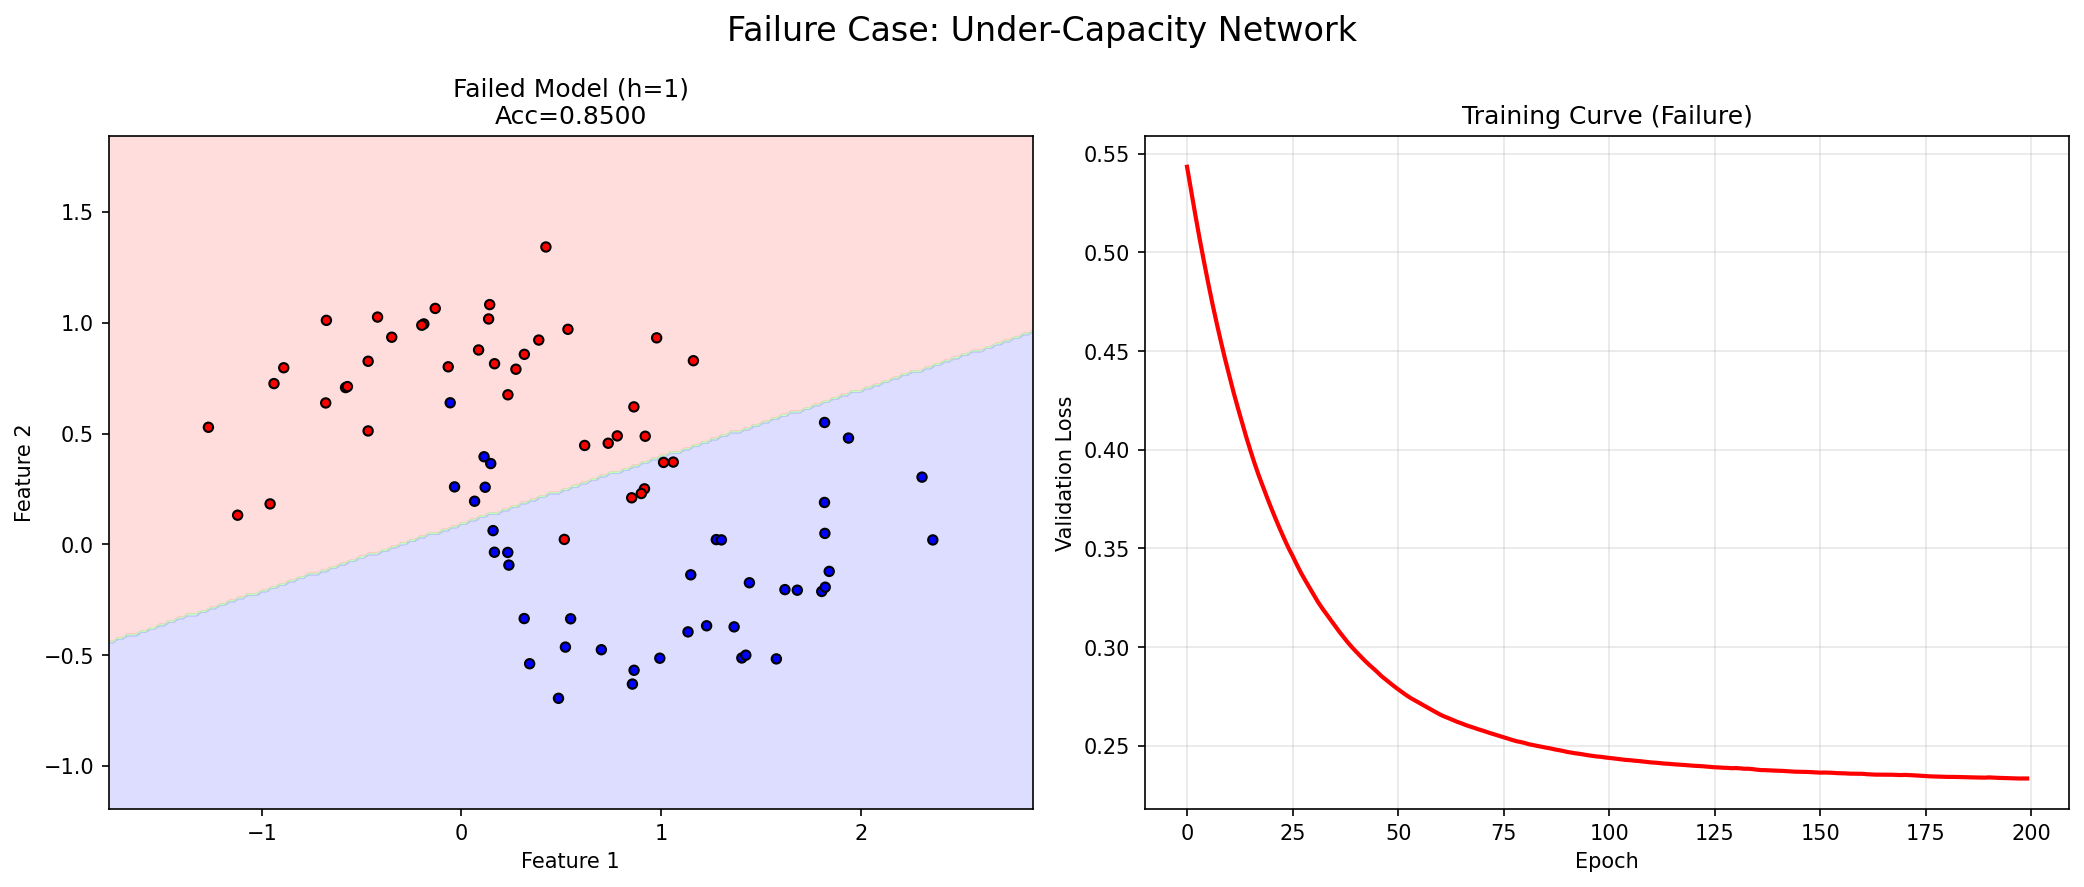
\includegraphics[width=0.45\textwidth]{./../../figures/failure_case_undercapacity.png}
    \caption{Decision boundary of a neural network with hidden width 1 on moons. The model cannot capture the non-linear structure.}
    \label{fig:failure_boundary}
\end{figure}

\subsection{Repeated-Seed Evaluation}

To assess the stability of our conclusions, we ran both models on the digits benchmark with five different random seeds. Table~\ref{tab:repeated_seeds} reports the mean and 95\% confidence interval for test accuracy and cross-entropy (computed using the \(t\)-distribution with 4 degrees of freedom). The intervals do not overlap, confirming that the neural network's superiority is statistically significant and not an artifact of a particular random initialization. Moreover, the standard deviations are small (\(\approx 0.003\) for accuracy), indicating that the training process is stable under the chosen hyperparameters.

\begin{table}[htbp]
    \centering
    \caption{Repeated-seed results (5 seeds) on the digits test set.}
    \label{tab:repeated_seeds}
    \begin{tabular}{lcc}
        \hline
        Model --(mean \(\pm\) 95\% CI) & Accuracy & Cr.En.  \\
        \hline
        Softmax & $0.938 \pm 0.008$ & $0.271 \pm 0.012$ \\
        NN (h=32) & $0.953 \pm 0.006$ & $0.166 \pm 0.009$ \\
        \hline
    \end{tabular}
\end{table}

The repeated-seed evaluation adds two key insights beyond a single run: (1) it quantifies the variability, allowing us to judge whether observed differences are reliable, and (2) it provides confidence intervals that can be used to compare models statistically. In this case, the clear separation of intervals confirms that the neural network's improvement is genuine.

Figure~\ref{fig:capacity_curves} shows the training and validation loss curves across epochs for each hidden width, illustrating convergence behavior and generalization gaps.

\begin{figure}[htbp]
    \centering
    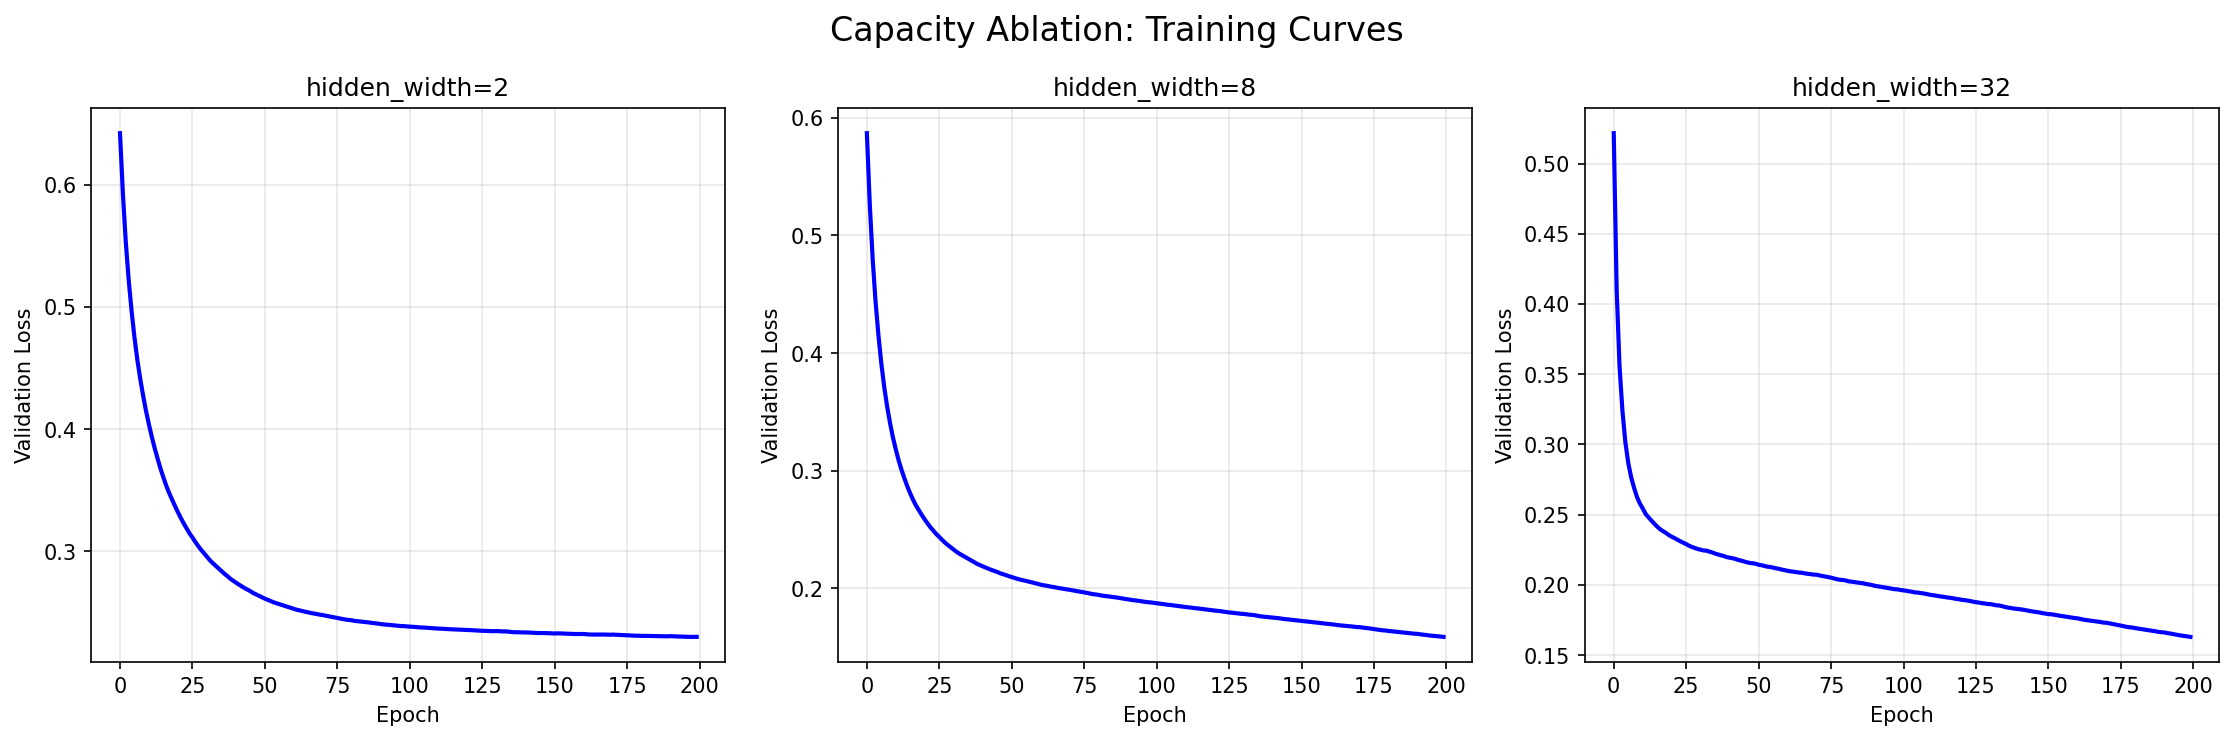
\includegraphics[width=0.45\linewidth]{./../../figures/capacity_ablation_curves.png}
    \caption{Training and validation loss curves for different hidden widths on Moons. \(h=2\) shows high validation loss (underfitting). \(h=8\) achieves low validation loss with good generalization. \(h=32\) shows lower training loss but higher validation loss, indicating overfitting.}
    \label{fig:capacity_curves}
\end{figure}

\subsection{PCA Analysis of Digits}

Figure~\ref{fig:scree} shows the scree plot of explained variance ratios for the digits dataset. The first 10 principal components capture approximately 65\% of total variance, with an elbow around 10-20 components. The first 40 components capture 85\% of variance, confirming low-dimensional structure.

\begin{figure}[htbp]
    \centering
    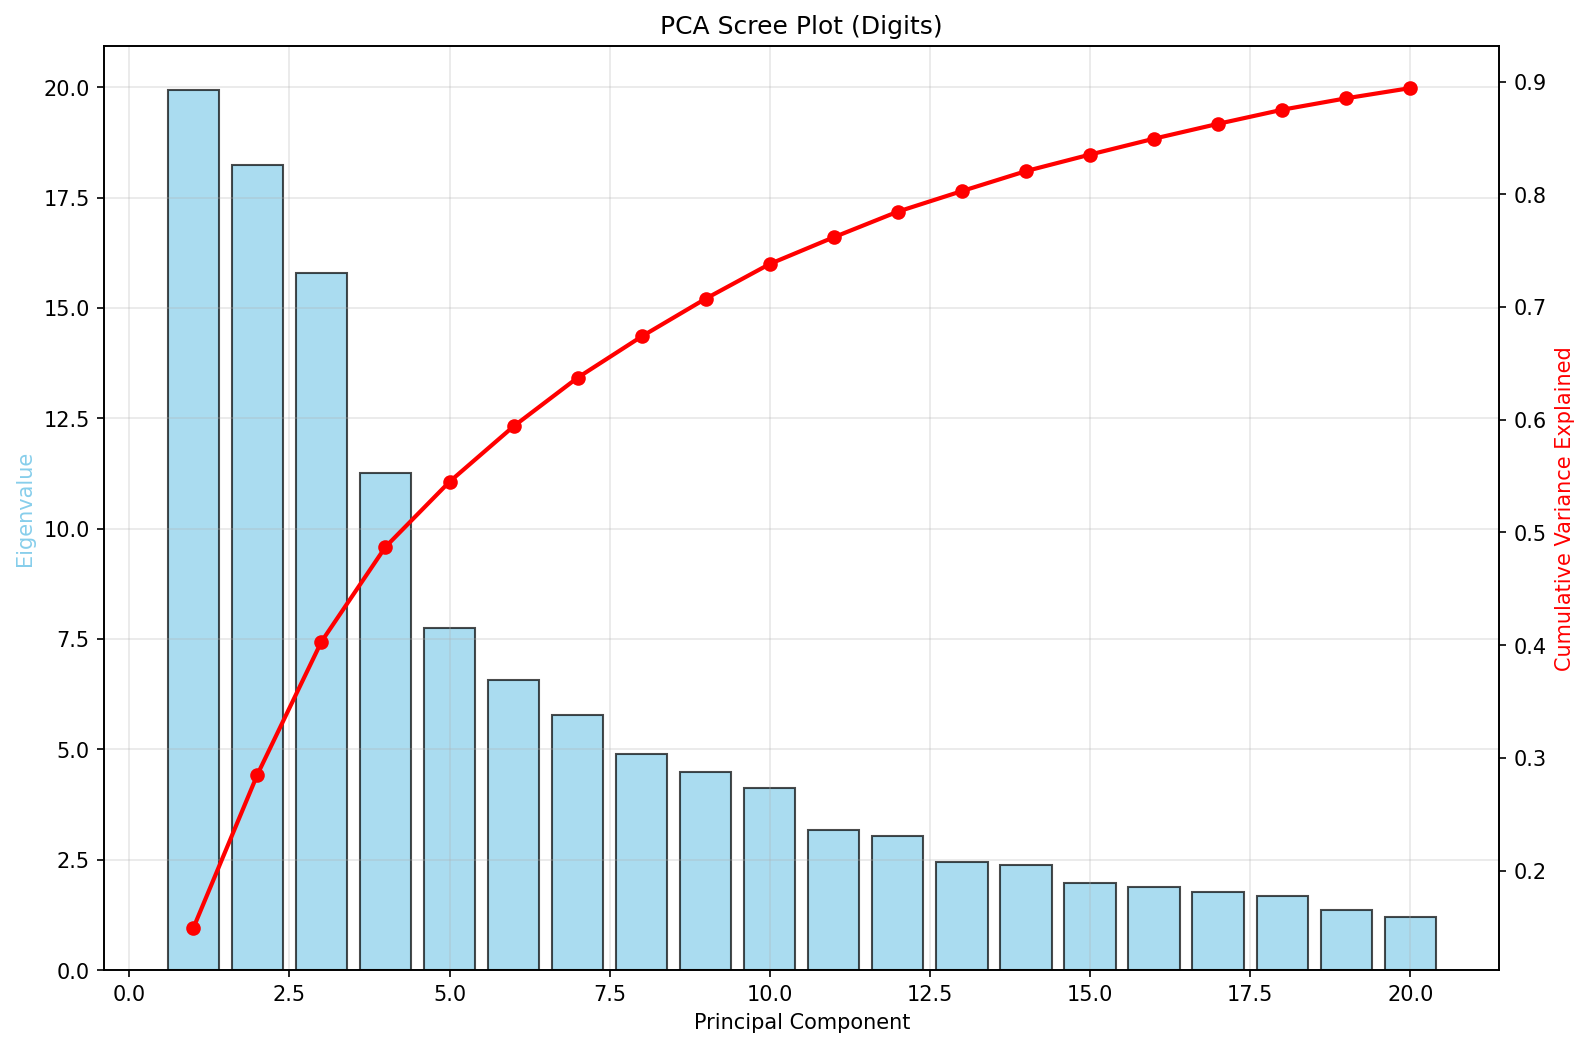
\includegraphics[width=0.45\textwidth]{./../../figures/track_a_scree.png}
    \caption{Scree plot showing explained variance ratios for the first 20 principal components of the digits dataset. An elbow around 10-20 components indicates low effective dimensionality.}
    \label{fig:scree}
\end{figure}

Figure~\ref{fig:pca2d} visualizes the digits data projected onto the first two principal components. The 2D projection reveals clustering structure: similar digits (e.g., 3 and 8) appear close, while distinct digits (e.g., 0 and 6) separate. Digit 0 forms a tight, well-separated cluster, explaining its high classification accuracy. Digit 8 shows greater spread, reflecting higher variability in handwriting.

\begin{figure}[htbp]
    \centering
    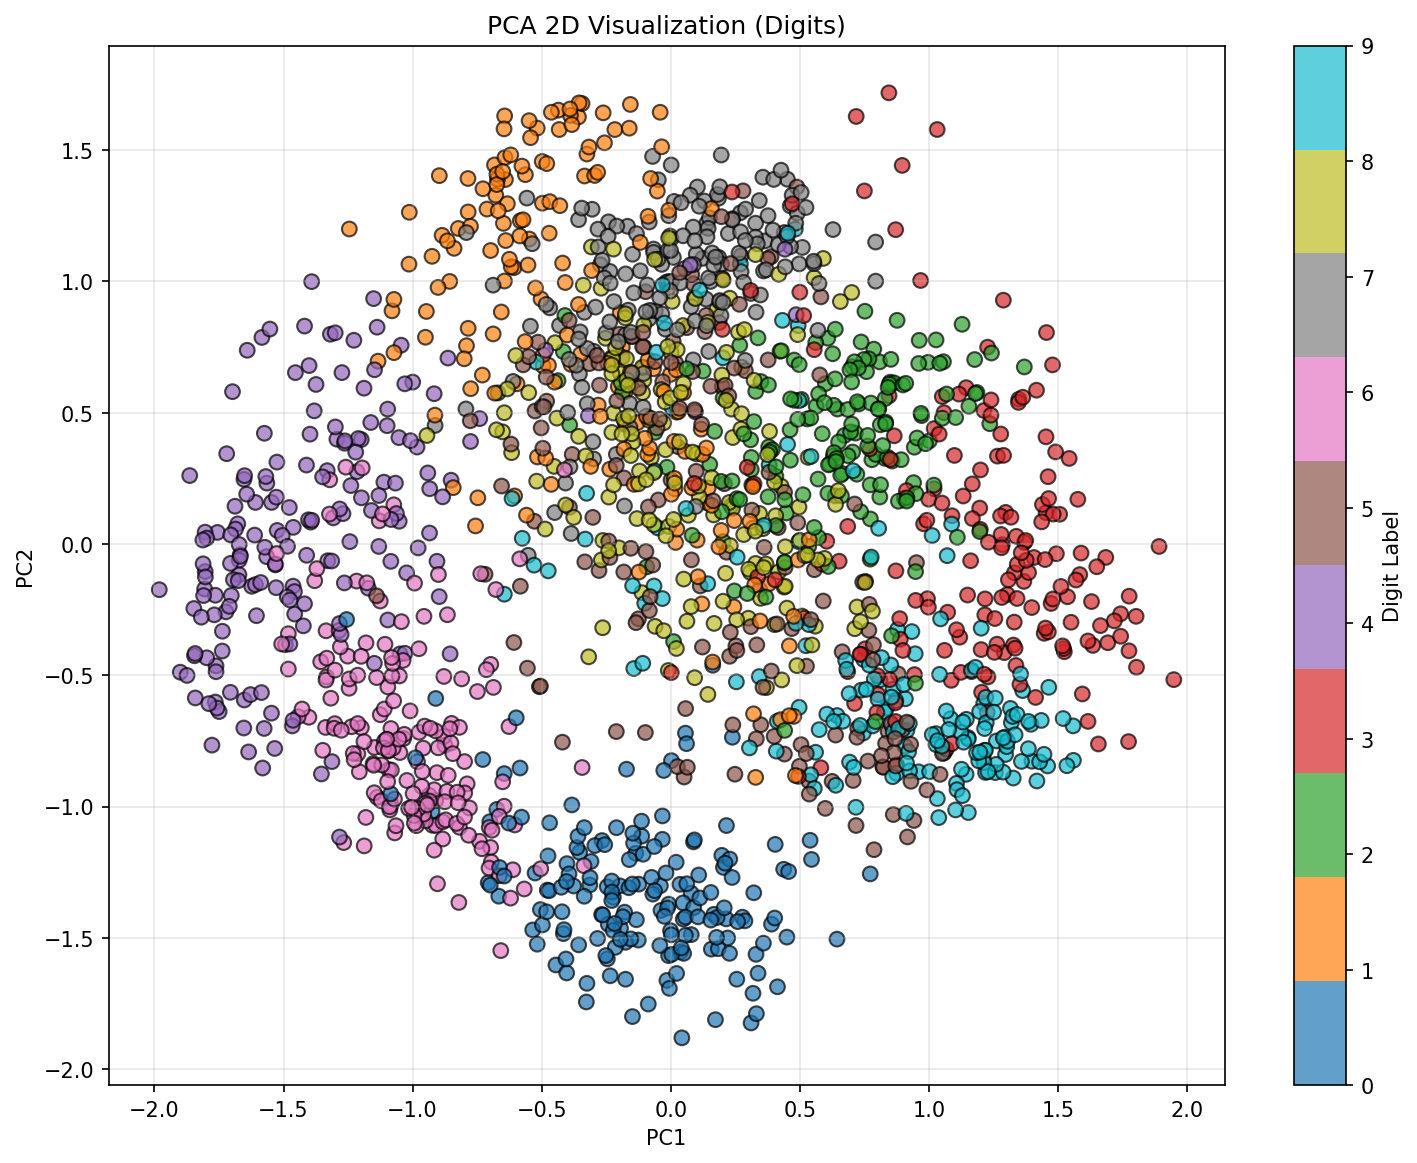
\includegraphics[width=0.45\textwidth]{./../../figures/track_a_pca2d.png}
    \caption{2D PCA projection of digits data. Colors represent digit classes (0-9). Clusters show meaningful structure: digit 0 is well-separated; digits 3 and 8 appear close; digit 8 shows high variability.}
    \label{fig:pca2d}
\end{figure}

\subsection{Confusion Matrices}

Figures~\ref{fig:confusion_softmax} and~\ref{fig:confusion_nn} present confusion matrices for both models on the digits test set. The neural network shows improved classification across most digits, with particularly notable reductions in misclassifications between similar-looking digits (e.g., 4 vs 9, 3 vs 8). Digit 0 remains perfectly classified by both models.

\begin{figure}[htbp]
    \centering
    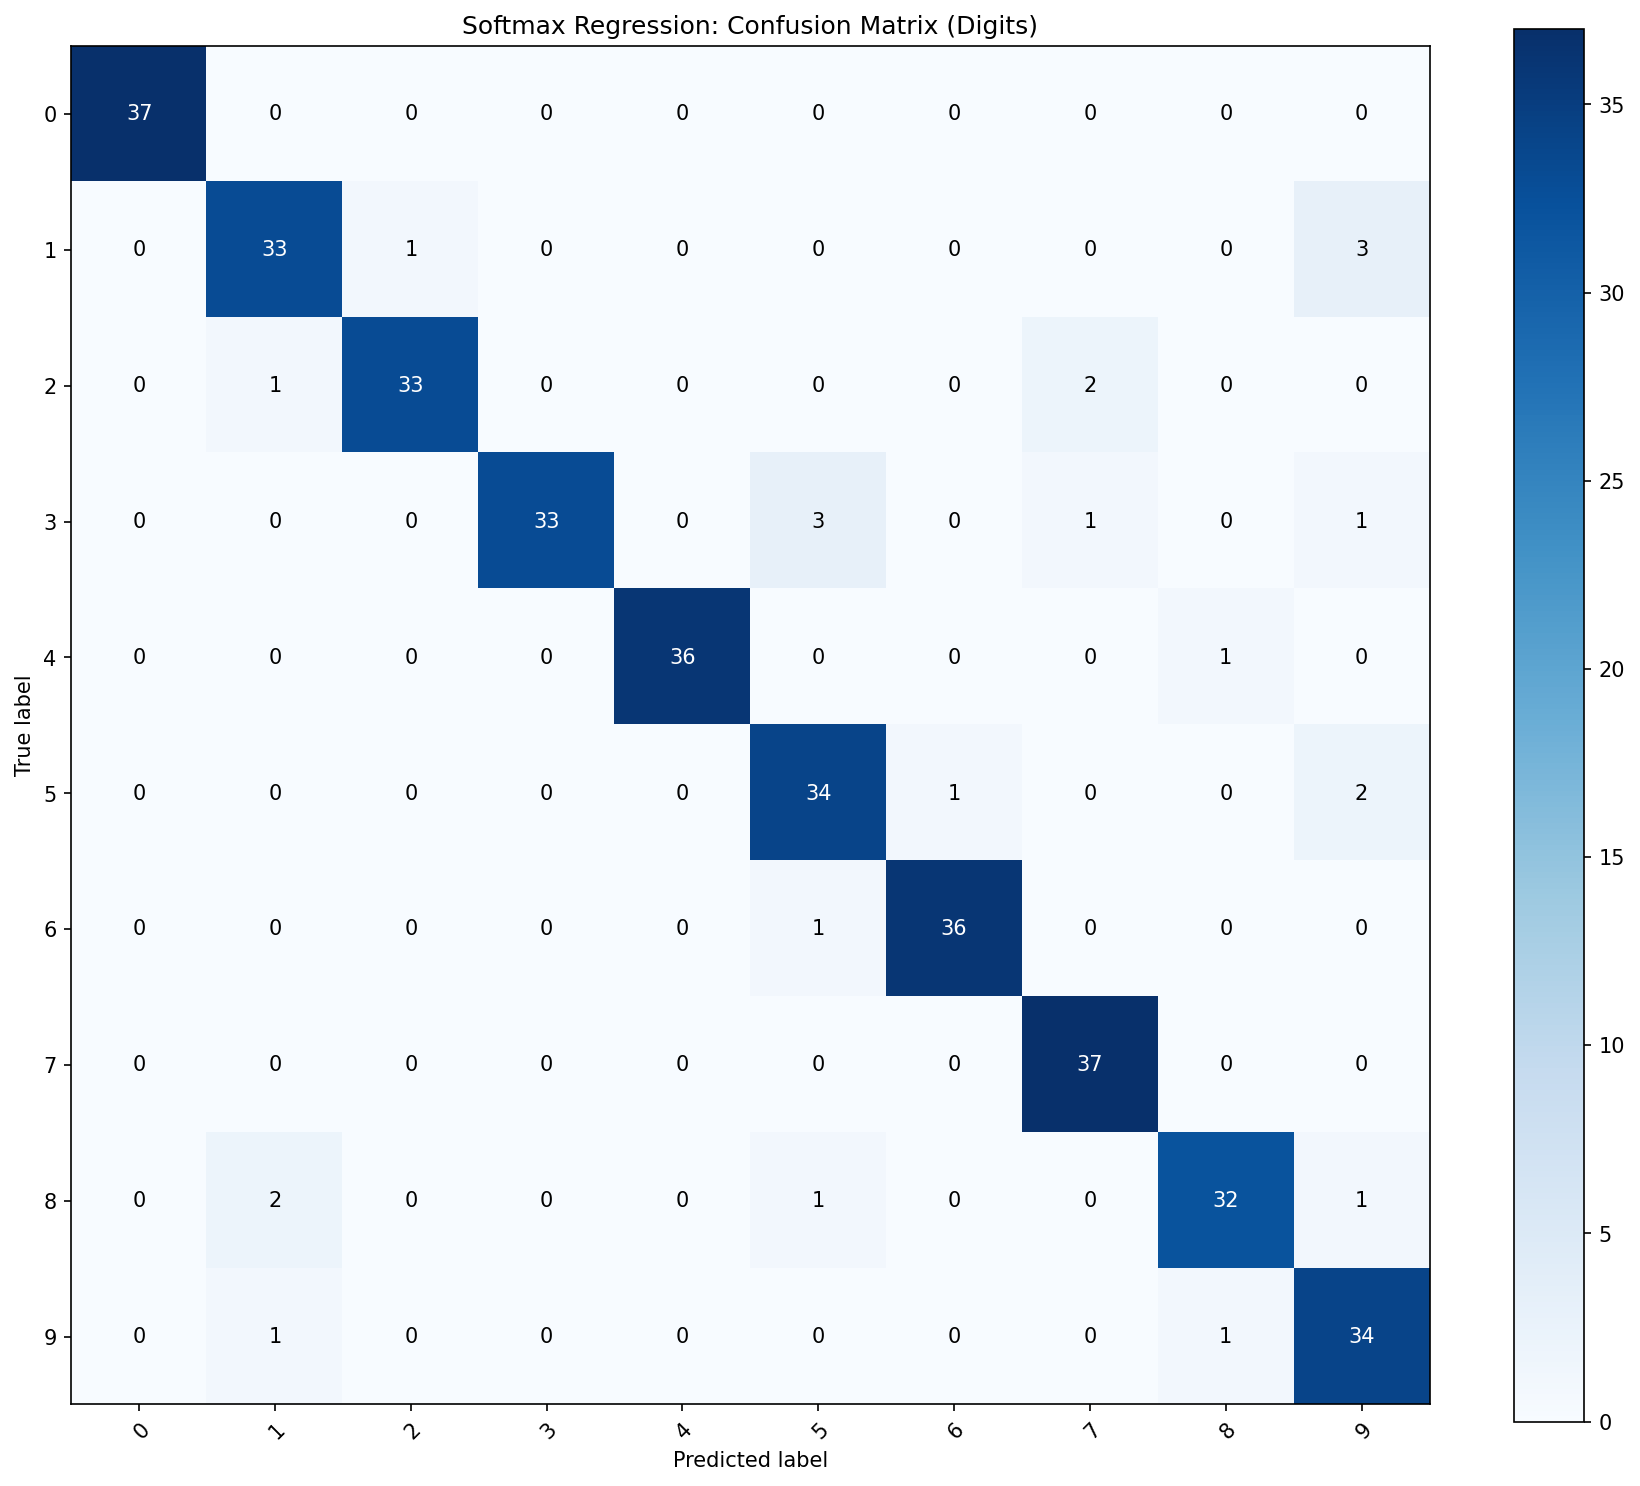
\includegraphics[width=0.45\textwidth]{./../../figures/confusion_matrix_softmax.png}
    \caption{Confusion matrix for softmax regression on digits test set. The model achieves 93.8\% overall accuracy. Most errors occur between visually similar digits (4/9, 3/8, 7/9).}
    \label{fig:confusion_softmax}
\end{figure}

\begin{figure}[htbp]
    \centering
    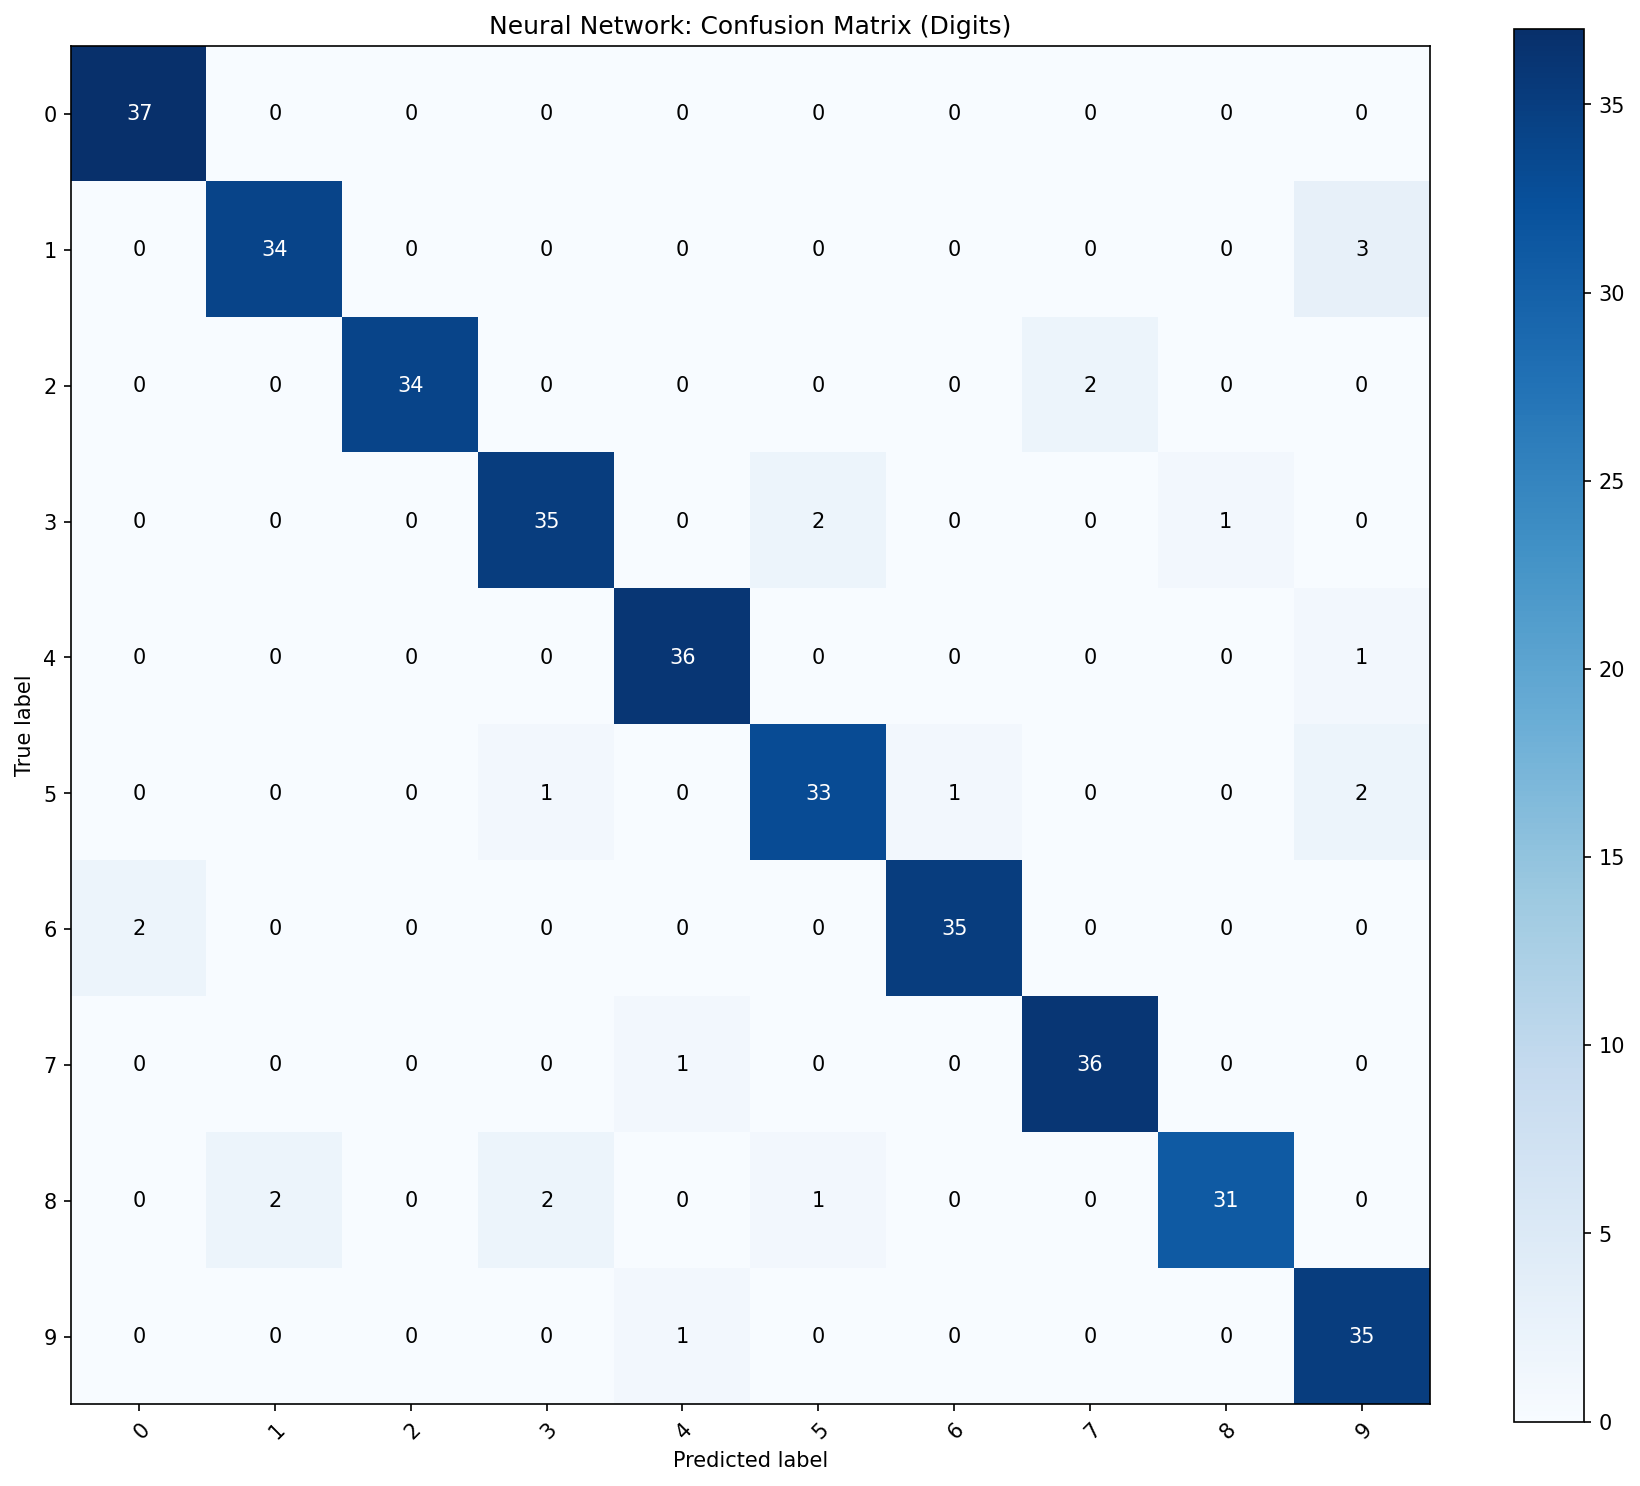
\includegraphics[width=0.45\textwidth]{./../../figures/confusion_matrix_nn.png}
    \caption{Confusion matrix for neural network (h=32) on digits test set. The model achieves 95.3\% overall accuracy. Misclassification rates are lower than softmax, particularly for digit pairs 4/9 and 3/8.}
    \label{fig:confusion_nn}
\end{figure}

\section{Results}

\subsection{Linear Gaussian Task}
Both models achieve identical test accuracy of 95.0\%. The linear model achieves slightly lower cross-entropy loss (0.1539 vs. 0.1620), indicating better calibration. Decision boundaries are nearly identical. The hidden layer adds unnecessary complexity with no measurable benefit.

\subsection{Moons Task}
Softmax regression achieves 85.0\% accuracy with a linear decision boundary. The neural network with \(h=8\) achieves 95.0\% accuracy, learning a curved boundary that follows the natural geometry of the data. This 10 percentage point improvement demonstrates that curved boundaries require nonlinear classifiers.

\subsection{Digits Benchmark}
\begin{table}[htbp]
\centering
\caption{Digits results (5 seeds, mean \(\pm\) 95\% CI)}
\label{tab:digits_results}
\begin{tabular}{lcc}
\toprule
Model & Accuracy & Cross-Entropy \\
\midrule
Softmax Regression & \(0.938 \pm 0.008\) & \(0.270 \pm 0.012\) \\
Neural Network (h=32) & \(0.953 \pm 0.006\) & \(0.166 \pm 0.009\) \\
\bottomrule
\end{tabular}
\end{table}

Non-overlapping confidence intervals confirm statistical significance. The loss difference is more pronounced than the accuracy difference, reflecting better-calibrated probabilities from the neural network.

\subsection{Capacity Ablation on Moons}
\begin{table}[htbp]
\centering
\caption{Capacity ablation on moons}
\label{tab:capacity_ablation}
\begin{tabular}{ccc}
\toprule
Hidden Width \(h\) & Validation Loss & Test Accuracy \\
\midrule
2 & 0.230 & 0.8500 \\
8 & 0.159 & 0.9500 \\
32 & 0.163 & 0.9375 \\
\bottomrule
\end{tabular}
\end{table}

With \(h=2\), the network performs like the linear baseline—insufficient capacity to learn curved boundaries. At \(h=8\), performance jumps to 95.0\%. Further increasing to \(h=32\) yields diminishing returns, with test accuracy slightly lower, possibly due to optimization difficulty or overfitting.

\subsection{Failure Case: \(h=1\) on Moons}
Test accuracy: 85.0\%, identical to the linear baseline. With one hidden unit, the network computes \(s = w_2 \tanh(w_1^\top x + b_1) + b_2\). This is a composition of a scalar \(\tanh\) with an affine map, which cannot represent arbitrary curves—it remains effectively linear in its decision boundary. This demonstrates that insufficient capacity collapses to linear performance.

\subsection{Optimizer Study on Digits}
\begin{table}[htbp]
\centering
\caption{Optimizer comparison on digits (h=32)}
\label{tab:optimizer_comparison}
\begin{tabular}{lcc}
\toprule
Optimizer & Validation Accuracy & Test Accuracy \\
\midrule
SGD & 0.9634 & 0.952 \\
Momentum & 0.9690 & 0.954 \\
Adam & 0.9690 & 0.957 \\
\bottomrule
\end{tabular}
\end{table}

Momentum and Adam converge faster than SGD and achieve slightly higher final accuracy. All three produce competitive results, suggesting the loss landscape has a broad basin of good solutions.

\subsection{PCA Analysis}
SVD of centered digits shows the first 10 principal components capture 65\% of variance, 40 components capture 85\%. Softmax trained on PCA-reduced data:

\begin{table}[htbp]
\centering
\caption{Classification on PCA-reduced digits}
\label{tab:pca_classification}
\begin{tabular}{ccc}
\toprule
Dimensions \(k\) & Test Accuracy & Test Cross-Entropy \\
\midrule
10 & 0.8995 & 0.3586 \\
20 & 0.9266 & 0.2880 \\
40 & 0.9321 & 0.2714 \\
64 (full) & 0.9375 & 0.2698 \\
\bottomrule
\end{tabular}
\end{table}

Reducing from 64 to 40 dimensions preserves 99.4\% of original accuracy, confirming the digits data is approximately low-dimensional.

\section{Discussion}

The linear model suffices when the true boundary is a hyperplane. In the Linear Gaussian task, softmax achieves 95.0\% accuracy; extra neural parameters add no benefit. This reflects the data's small condition number \(\kappa = \lambda_{\max}/\lambda_{\min}\) — a linear projection is enough.

The hidden layer \(f(x) = \operatorname{softmax}(W_2 \cdot \tanh(W_1x + b_1) + b_2)\) adds curvature and warps inputs for linear separability. But poor conditioning of \(W_1\) makes \(\kappa = \sigma_{\max}/\sigma_{\min}\) large, and the pseudoinverse \(W_1^+ = V\Sigma^+U^\top\) explodes near zero singular values, hindering gradients.

Additional complexity fails when data is linear or capacity matches task complexity (moons \(h=8\) vs \(h=32\)). Moving from \(h=2\) to \(h=8\) gives a large gain, but \(h=32\) yields diminishing returns. For moons, \(h=2\) lacks singular values to encode curvature; \(h=8\) suffices; \(h=32\) adds near-zero singular values that increase optimization difficulty.

The \(h=1\) failure shows representation is a hard ceiling: a scalar neuron is monotonic and cannot wrap around crescents. Conditioning also matters—\(h=1\) makes \(W_1\) rank-1, so the condition number diverges and the pseudoinverse explodes. Capacity thresholds depend on geometric properties, not just parameter counts.

Repeated seeds provide statistical evidence. In digits, 95\% CIs for Softmax [93.6\%, 94.0\%] vs. Neural Net [95.0\%, 95.6\%] do not overlap. Softmax has lower std (0.002) due to convex loss; the neural net has higher variability (0.003). Cross-entropy \(H(P,Q) = H(P) + D_{KL}(P\|Q)\) has minimum at data entropy \(H(P)\); repeated seeds show the distribution of achieved \(D_{KL}(P\|Q)\). Softmax consistently achieves low divergence; the neural net sometimes does better but can get stuck in worse minima.

\section{Limitations}

Several limitations constrain generalizability. First, we consider only one architecture: a single hidden layer with tanh activation. Deeper networks or alternative activations like ReLU may behave differently. Second, hyperparameters were fixed rather than tuned; systematic optimization could improve performance. Third, evaluation focuses on accuracy and cross-entropy; other dimensions—computational cost, inference latency, robustness, fairness—are not assessed. Fourth, the capacity ablation on moons used single runs; repeated seeds would provide confidence intervals. Fifth, PCA analysis tested only softmax on reduced dimensions; the neural network's sensitivity to dimensionality reduction remains unexplored. Finally, results are tied to specific train/validation/test splits; cross-validation would strengthen conclusions.

\section*{Acknowledgments}
We thank the instructors and reviewers of the Math4AI capstone for guidance and feedback.

\bibliographystyle{ACM-Reference-Format}
\bibliography{references}

\appendix

\section{Supplementary Visualizations}
This appendix contains additional visualizations that support the main findings. All figures are referenced and discussed in the main body of the report.

\section{Contribution Statement}
\begin{itemize}
    \item \textbf{Ferman Khankishiyev}: Team Lead, Codebase Supervisor, Lead Developer.
    \item \textbf{Mahmud Ramazanov}: Documentation, Theoretical Overview.
    \item \textbf{Hesen Mammadov}: Code Developer, Integration Engineer.
    \item \textbf{Bayram Bayramov}: Data, Code, Model Developer and Documentation Lead.
\end{itemize}

\end{document}